\documentclass{standalone}
\usepackage{tikz}
\usetikzlibrary{patterns}
\usetikzlibrary{positioning}
\usetikzlibrary{patterns, positioning}
\usetikzlibrary{shapes.misc}
\usepackage[outline]{contour}
\contourlength{1.5pt} 
\usepackage[sfdefault]{ClearSans}

\begin{document}
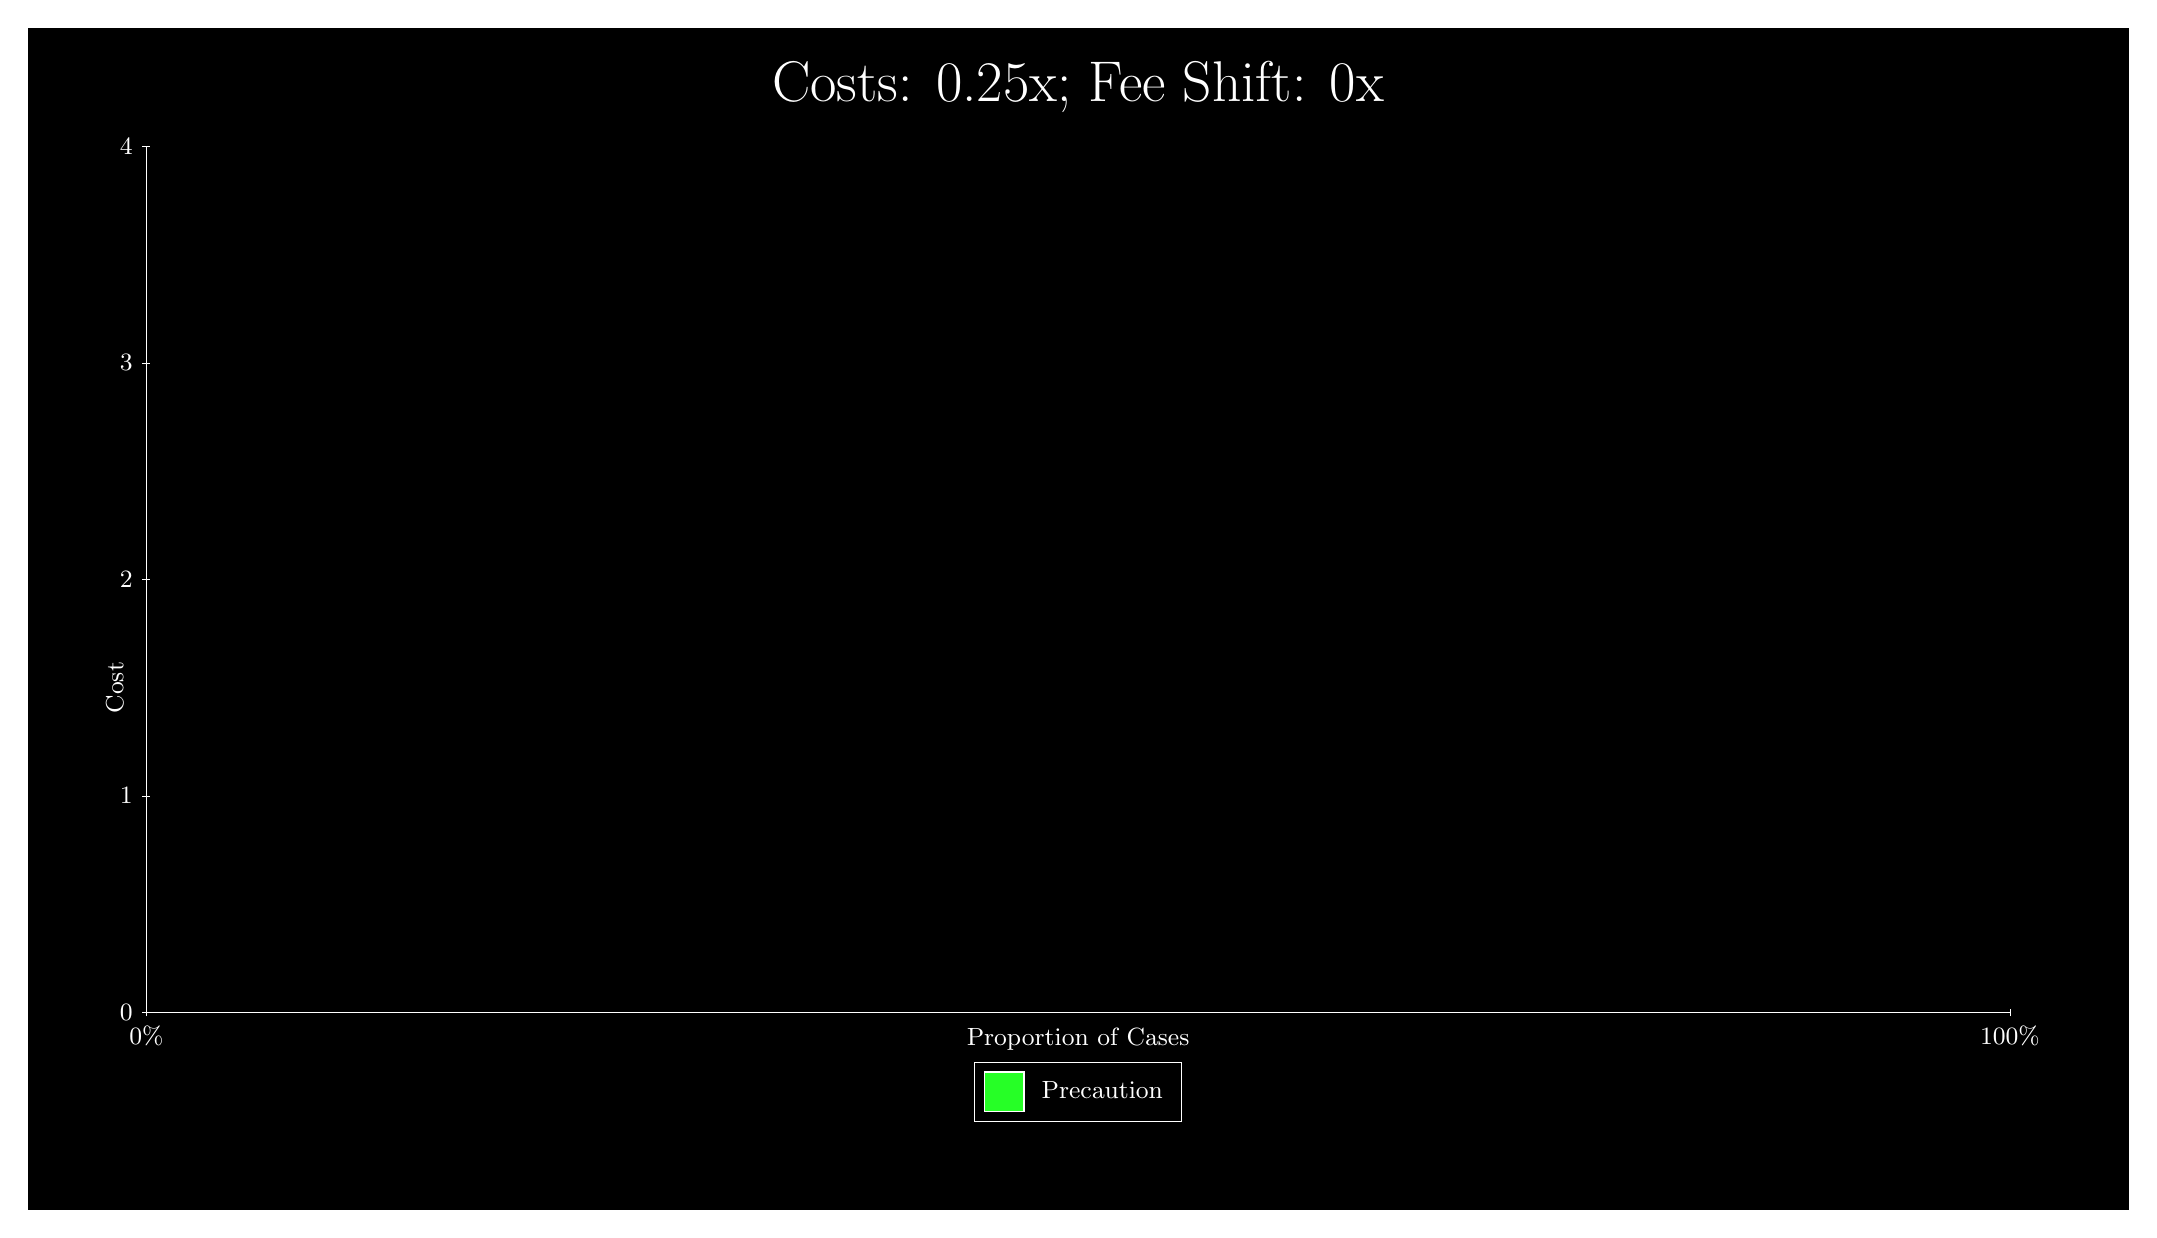
\begin{tikzpicture}
\draw[fill=black] (0,0) rectangle (26.667,15);
\draw[draw=none,text=white] (0,13.5) rectangle (26.667,15) node[midway] {\huge Costs: 0.25x; Fee Shift: 0x };
\draw[fill=green!85,draw=white,very thin] (1.5,2.5) rectangle (25.167,2.5027);
\draw[white,very thin] (1.5,2.5) -- (1.5,13.5);
\node[font=\small,rotate=90,text=white, anchor=center] at (1.1, 6.625) {Cost};
\draw[white,very thin] (1.45,2.5) -- (1.55,2.5);
\node[font=\small,text=white, anchor=east] at (1.45, 2.5) {0};
\draw[white,very thin] (1.45,5.25) -- (1.55,5.25);
\node[font=\small,text=white, anchor=east] at (1.45, 5.25) {1};
\draw[white,very thin] (1.45,8) -- (1.55,8);
\node[font=\small,text=white, anchor=east] at (1.45, 8) {2};
\draw[white,very thin] (1.45,10.75) -- (1.55,10.75);
\node[font=\small,text=white, anchor=east] at (1.45, 10.75) {3};
\draw[white,very thin] (1.45,13.5) -- (1.55,13.5);
\node[font=\small,text=white, anchor=east] at (1.45, 13.5) {4};

\draw[white,very thin] (1.5,2.5) -- (25.167,2.5);
\node[font=\small,text=white, anchor=south] at (13.333, 1.9) {Proportion of Cases};
\draw[white,very thin] (1.5,2.45) -- (1.5,2.55);
\node[font=\small,text=white, anchor=north] at (1.5, 2.45) {0\%};
\draw[white,very thin] (25.167,2.45) -- (25.167,2.55);
\node[font=\small,text=white, anchor=north] at (25.167, 2.45) {100\%};

\draw (13.3333,2.5) node (B) {};
\begin{scope}[align=center]
\matrix[scale=0.5,draw=white,below=0.5cm of B,nodes={draw},column sep=0.1cm]{
\node[rectangle,draw,minimum width=0.5cm,minimum height=0.5cm,fill=green!85]{}; & \node[draw=none,font=\small,text=white]{Precaution}; \\\\
};\end{scope}

\end{tikzpicture}
\end{document}